\section{Time / Complexity tradeoffs}
\label{2406:sec:main:cold_start}
In this section, we characterize the intertwined dependence between the batch size and the hardness of the learning task in determining the number of one-pass SGD iterations needed to achieve weak recovery of the teacher subspace as in Definition~\ref{2406:def:weak_recovery}. We offer a detailed picture of the tradeoffs to consider in order to minimize the training iteration time $T$, compactly illustrated in the phase diagram in Figure~\ref{2406:fig:cold_start_pd}.


\paragraph{Network initialization ---}
We consider random initialization for the hidden layer weights of the network~\eqref{2406:eq:main:newtwork_def}, while the second layer weights are kept fixed:
\begin{align}\label{2406:eq:initial_conditions_unconstrainted}
    \vec w_{j,0}\sim \mathrm{Unif}(\mathbb{S}^{d-1}),\quad a_{j,0} = 1 \qquad j \in [p].
\end{align}
We will refer to this situation as \emph{cold start}, since the initial network correlation with the target directions is vanishing when \(d\to+\infty\). 

\paragraph{Generalized Linear Models ---}
The seminal work of \cite{arous2021online} studies the weak recovery problem for Generalized Linear Models (GLMs), i.e. $p=1$, when learning single-index targets ($k=1$). Starting from randomly initialized networks as defined in~\eqref{2406:eq:main:newtwork_def}, the time iterations needed for one-pass SGD (with one sample per batch) to achieve weak recovery of the target direction respects:
\begin{align}
\label{2406:eq:main:time_complexity_single_index}
    I(\ell) =
    \begin{cases}
        &O(d^{\ell -1} ) \qquad \text{if $\ell>2$} \\
        &O(d \log{d} ) \qquad \text{if $\ell=2$} \\
        &O(d) \qquad \text{if $\ell=1$}
    \end{cases}
\end{align}
where $\ell$ is the information exponent of the target $f_\star$. 

As far as weak recovery of the target subspace is concerned, the characterization of multi-index targets follows the same lines of thought just replacing the information exponent by the leap index of the target, e.g. see Definition~\textbf{3} of \cite{dandi2023how} or Definition~\textbf{1} of \cite{abbe2023sgd}. 
Similarly to the information exponent definition, the leap index is the lowest rank of the tensors appearing in the Hermite expansion of the target $f^\star$. 
Therefore, we choose to study in the following the training dynamics for the $p=k=1$ scenario for general batch sizes $n_b$. 
This assumption is useful to provide rigorous guarantees as it largely reduces the complexity of the projected SGD dynamics. However, we argue (supported by numerical simulations in Appendix~\ref{2406:app:multiindex_model}) that the same phenomenology will hold for larger values of $p$ and $k$. 


\subsection{Weak recovery with one-pass SGD}
Consider the gradient descent dynamics defined on the hidden layer weights by Equation~\eqref{2406:eq:main:gd_update_weights}. We focus on the description of the time evolution of the correlation between the network's hidden layer weight and the target direction:
\begin{align}
    m_t= \langle \vec w_t , \vec w^\star \rangle 
\end{align}
Our first main result is to characterize the time to achieve weak recovery of the target direction $\vec w^\star$ as a function of the batch size and the information exponent of the target. We make very weak assumptions on the activation and labeling functions, namely only assuming a sub-polynomial growth:
\begin{assumption}[Polynomial growth]\label{2406:assump:poly_growth}
    The activation function $\sigma$ is differentiable everywhere, except maybe at a finite set of points. Both $\sigma'$ and $f^\star$ are sub-polynomial, i.e. there exists a $q > 0$ and a constant $C$ such that for any $x\in \mathbb R$
    \begin{equation}
        |\sigma'(x)|\leq C(1+x)^q \quad \text{and} \quad |f^\star(x)|\leq C(1+x)^q
    \end{equation}
\end{assumption}

\begin{assumption}[Well-posedness]\label{2406:assump:well_posed}
    Let $(c_k)_{k \geq 0}$ and $(c_k^\star)_{k\geq 0}$ be the Hermite coefficients of $\sigma$ and $h^\star$, respectively. Then $c_\ell \neq 0$, and if $\ell$ is even, then $c_\ell c_\ell^\star > 0$.
\end{assumption}

\begin{assumption}[Initialization]\label{2406:assump:init}
    There exists a $\kappa > 0$ such that $m_0 > \kappa / \sqrt{d}$. Further, if $\ell$ is odd, then $m_0$ is such that
    \[ c_\ell c_\ell^\star m_0 > 0 \]
\end{assumption}
Assumption 2 ensures that the optimization problem is achievable for gradient flow on the population loss $\mathcal{R}$. Indeed, one can show that when $m \approx 0$,
\[ \mathcal{R} = 2(1 - c_\ell c_\ell^\star m^\ell) + o(m^\ell); \]
as a result, if $\ell$ is even and $c_\ell c_\ell^\star < 0$, then $m = 0$ is a local maximum of $\mathcal{R}$ and weak recovery is impossible. When $\ell$ is odd, the point $m=0$ is always a strict saddle, so Assumption~\ref{2406:assump:init} ensures that we start on the correct side of the saddle. Under the initialization scheme described by Equation~\ref{2406:eq:initial_conditions_unconstrainted}, the first condition is satisfied with arbitrarily high probability upon decreasing $\kappa$, while the second is a $1/2$-probability event.

We are now in the position to formally state the result:
\begin{theorem} [Projected SGD weak recovery]
\label{2406:thm:main:sgd_weak_recovery}
   Consider the projected SGD algorithm with square loss  (Equations~\eqref{2406:eq:main:gd_update_weights}, \eqref{2406:eq:main:projected_sgd}), and suppose that Assumptions~\ref{2406:assump:poly_growth}-\ref{2406:assump:init} hold. There exist absolute constants $c_\gamma, C_\gamma$ such that if
   \[ \gamma\leq c_\gamma \min\left(1, n_b d^{-\left(\frac\ell2\vee 1\right)} \log(d)^{-C_\gamma}\right), \]
    then for large enough $d$ we have with probability $1-ce^{-c\log(n)^2}$
   \begin{equation}
       t_\eta^+ \leq C\gamma^{-1}d^{\left(\frac{\ell}2 - 1 \right) \vee 0}\log(d).
   \end{equation}
\end{theorem}



 
 \subsection{Illustration of Theorem~\ref{2406:thm:main:sgd_weak_recovery}} The phase diagram in Figure~\ref{2406:fig:cold_start_pd} exemplifies Theorem~\ref{2406:thm:main:sgd_weak_recovery}. We identify three \textit{learning phases}: SGD learning, Correlation Loss SGD learning, and SGD impossible. These regions are explored by varying the batch size and learning rate exponents $\delta,\mu$. Our theory characterizes the optimal learning rate to achieve the lowest possible time iterations of SGD to weakly recover the target direction $\vec w^\star$ when the batch size respects $n_b = o(d^{\ell -1})$:
 \begin{align}
     \delta^\star(\mu) = 
     \begin{cases}
         &\frac{\ell}{2} - \mu  \qquad \text{if} ~ ~ \mu< \sfrac{\ell}{2} \\
         & 0 \qquad \qquad \text{otherwise} 
     \end{cases}
 \end{align}
 
\textbf{Weak recovery region ---} In the region $n_b \lesssim d^{\sfrac{\ell}{2}}$ there is a net benefit in using larger batch sizes in the SGD optimization. 
This section shows a similar phenomenology to \cite{arous2021online}: if we optimally choose the learning rate exponent $\delta^\star(\mu)$, the number of time iterations needed to weakly recover the teacher direction $\vec w^\star$ is simply $T(n_b) = \sfrac{I(\ell)}{n_b}$, rescaling straightforwardly the time complexity of the $n_b=1$ case in Equation~\eqref{2406:eq:main:time_complexity_single_index}. By considering higher values for the learning rate ($\delta < \delta^\star(\mu)$) SGD is not able to weakly recover the signal as the dynamics is dominated by terms contracting the network~/~target correlation to zero, defining the SGD impossible region. Vice versa, if one takes into account lower learning rates ($\delta > \delta^\star(\mu)$), it is certainly possible to weakly-recover the target, but at a higher time complexity cost. 

\textbf{Self-interaction regime --- } Conversely, the region $d^{\sfrac{\ell}{2}} \ll n_b \lesssim d^{\max (\ell-1,1)}$ does not adhere to the same straightforward paradigm. 
% The dynamics of weights norm is dominated by a \textit{ self-interaction term } leading to the \emph{Correlation Loss SGD} region. 
Indeed, standard SGD is not able to achieve weak recovery of the teacher direction using $T(n_b)  =  \sfrac{I(\ell)}{n_b}$ time iterations, but a simple modification of it - that we call \emph{Correlation Loss SGD} - is able to. The number of steps needed to weakly recover the target with this new training protocol can then be pushed down to \(T=\mathrm{polylog}(d)\) when using batch sizes $n_b = O(d^{\max (\ell-1,1)})$. We refer to the next section for a detailed analysis of this regime.
 % \\ \textbf{Sub-power region ---} If $n = \omega(d^{\ell-1})$ Theorem \ref{2406:thm:main:sgd_weak_recovery} does not offer a sharp characterization of this region. 
 
\textbf{One-step regime ---} Recent works have discussed the role of one large learning rate gradient descent step (\textit{giant step}) when training of two-layer networks \citep{ba2022high,damian2022neural,dandi2023how}. More precisely, \cite{dandi2023how} sharply characterizes the section $n_b = \Omega(d^{\ell})$ where it is possible to learn the teacher direction in just one step by setting the learning rate to $\delta_{\rm{giant-step}}(\mu) = \frac{1-\ell}{2}$. 



\subsection{The self-interaction regime}
Surprisingly, when the learning rate becomes extensive ($\gamma = \omega(1)$), the usual SGD algorithm struggles to achieve weak recovery. This can be explained by writing the gradient update as
\[ \vec{w}_t - \gamma \vec{g}_t = (1 - \gamma\langle \vec{g}_t, \vec{w}_t \rangle)\vec{w}_t - \gamma\vec{g}_t^\bot, \]
where $\vec{g}_t, \vec{g}_t^\bot$ are the gradient at time $t$ and its component orthogonal to $\vec{w}_t$, respectively. As a result, projected gradient descent can be seen as a version of spherical SGD with a random weight decay $\gamma \langle \vec{g}_t, \vec{w}_t \rangle$. When $\gamma = \omega(1)$, this weight decay also becomes of order $\omega(1)$, which leads to very unpredictable behavior of the process $(\vec{w}_t)_{t \geq 0}$.

 In this section, we study a modified version for the training protocol, in which the self-interaction term $\langle \vec{g}_t, \vec{w}_t \rangle$ is much smaller; we will refer to this new algorithm as \emph{Correlation loss SGD} (see e.g. \cite{damian2023smoothing}), as it effectively amounts to gradient updates on the correlation loss:
\begin{align} \label{2406:eq:main:correlation_loss}
\Tilde{\ell} = \frac{1}{n_b}\sum_{\nu \in [n_b]} 1-y^{\nu}f(\vec z^{\nu})
\end{align}

The above-described protocol is equivalent to consider a vanishing initialization scale for the second layer weights $\vec a_0$ of the network~\ref{2406:eq:main:newtwork_def}. Such assumptions are often considered in different theoretical efforts (see e.g. \cite{abbe2022merged,berthier2023learning,abbe2023sgd}). However, Figure~\ref{2406:fig:cold_start_pd} illustrates that a careful analysis of the initialization scale $\vec a_0$ is needed to paint an exhaustive description of the SGD dynamics. Indeed, considering Correlation loss SGD allows to overcome the limitations highlighted by Theorem~\ref{2406:thm:main:sgd_weak_recovery} for projected SGD. In particular, Correlation loss SGD is able to access the yellow region depicted in Figure~\ref{2406:fig:cold_start_pd} where the time complexity can be reduced again to $\Tilde{T}(n_b) = \sfrac{I(\ell)}{n_b}$ using the optimal learning rate $\Tilde{\delta}^\star(\mu) = \sfrac{\ell}{2} - \mu$ even for $\mu > \sfrac{\ell}{2}$. This is precisely stated in the following theorem. 
\begin{theorem} [\emph{Correlation Loss SGD} weak recovery]
\label{2406:thm:main:no_yhat_weak_recovery}
   Consider the projected SGD algorithm with correlation loss (Equations~\eqref{2406:eq:main:gd_update_weights}, \eqref{2406:eq:main:correlation_loss}), and suppose that Assumptions~\ref{2406:assump:poly_growth}-\ref{2406:assump:init} hold. There exists absolute constants $c_\gamma, C_\gamma$ such that if
   \[ \gamma \leq c_\gamma \log(d)^{-C_\gamma} \min\left( n_b d^{-\left(\frac\ell2\vee 1\right)}, \sqrt{\frac{n_b}d} \right) \]
    
   Then if $d$ is large enough, we have with probability $1-ce^{-c\log(n)^2}$
   \begin{equation}
      t_\eta^+ \leq C \max\left(1, \gamma^{-1}d^{\left(\frac{\ell}2 - 1 \right) \vee 0}\log(d)\right).
   \end{equation}
\end{theorem}
 The derivation of Theorems~\ref{2406:thm:main:sgd_weak_recovery} and \ref{2406:thm:main:no_yhat_weak_recovery} generalizes \cite{arous2021online} which studies the $n_b =1$ case. Informally, the result is obtained by analyzing the stability of the equation for the correlation \(m_t\), along with the requirement on the step-size for the suppression of the effects of the noise across time. However, there is a major difficulty introduced by the large step-size regime: when the gradient updates become larger, the Taylor-inspired bounds used in \cite{arous2021online} become vacuous. We work around this problem by showing that in this regime, there is a \emph{one-step improvement} which jumps directly to meaningful correlation with the target vector. All details can be found in Appendix~\ref{2406:sec:app:proofs}. We provide in Table~\ref{2406:table:weak_recovery} a representative summary of the results in Theorems~(\ref{2406:thm:main:sgd_weak_recovery}.~\ref{2406:thm:main:no_yhat_weak_recovery}) characterizing the time/complexity tradeoffs to achieve weak recovery of general single index target $f^\star$.
 \begin{table*}
\begin{center}
\setlength{\tabcolsep}{5pt}
\setlength\extrarowheight{5pt}
\begin{tabular}{c| c | c | c |c}
  \multirow{2}{*}{$\ell$} & SGD & SGD & Correlation loss SGD & One step  \\
  &{\scriptsize with $n_b \lesssim d^{\sfrac{\ell}{2}}$} &{\scriptsize with $d^{\sfrac{\ell}{2}} \ll n_b \lesssim d^{\max (\ell-1,1)}$} &{\scriptsize with $n_b=o\left(d^{\max(\ell-1, 1)}\right)$} &{\scriptsize with $n_b = O(d^\ell)$} \\
 \hline  $1$ & $\begin{array}{@{}l@{}} T = O(\sfrac{d}{n_b}) \\[2pt] N = O(d) \end{array}$ & $\begin{array}{@{}l@{}} T = O(1) \\[2pt] N = O(d) \end{array}$ & $\begin{array}{@{}l@{}} T = O(\sfrac{d}{n_b}) \\[2pt] N = O(d) \end{array}$ & $\begin{array}{@{}l@{}} T = 1 \\[2pt] N = O(d) \end{array}$ \\
 \hline  $2$ & $\begin{array}{@{}l@{}} T = O(\sfrac{d \log{d}}{n_b}) \\[2pt] N = O(d \log{d}) \end{array}$ & $\begin{array}{@{}l@{}} T = O(\log{d}) \\[2pt] N = O(d \log{d}) \end{array}$ & $\begin{array}{@{}l@{}} T = O(\sfrac{d\log{d}}{n_b}) \\[2pt] N = O(d \log{d}) \end{array}$ & $\begin{array}{@{}l@{}} T = 1 \\[2pt] N = O(d^2) \end{array}$ \\
 \hline
 $>2$ & $\begin{array}{@{}l@{}} T = O(\sfrac{d^{\ell -1}}{n_b}) \\[2pt] N = O(d^{\ell-1}) \end{array}$ & $\begin{array}{@{}l@{}} T = O(d^{\sfrac{\ell}{2} - 1}) \\[2pt] N = O(n_b d^{\sfrac{\ell}{2} - 1}) \end{array}$ & $\begin{array}{@{}l@{}} T = O(\sfrac{d^{\ell-1}}{n_b}) \\[2pt] N = O(d^{\ell-1}) \end{array}$ & $\begin{array}{@{}l@{}} T = 1 \\[2pt] N = O(d^{\ell}) \end{array}$ \\
 \hline
\end{tabular}
\caption{\textbf{Time~/~Complexity tradeoffs:} Number of iterations $T$ and the total number of samples $N$ needed to achieve weak recovery of the target for different training protocols in high dimensions. \textbf{Left:} One-pass SGD of batch size $n_b = d^{\sfrac{\ell}{2}}$, in this regime the optimal time complexity is obtained rescaling by $n_b$ the result of \cite{arous2021online} for $n_b=1$, i.e. by choosing the optimal learning rate $\gamma = O(n_b d^{-\sfrac{\ell}{2}})$. \textbf{Center-left:} One-pass SGD with batch size $d^{\sfrac{\ell}{2}} <  < n_b \lesssim d^{\max (\ell-1,1)}$, for hard problems ($\ell > 2$) the sample complexity is significantly increased with respect to the $n_b=1$ case up to $N = O(n_bd^{\sfrac{\ell}{2}-1})$. The learning rate cannot be increased proportionally to $n_b$ in this region, fixed to be $\gamma = O(1)$. \textbf{Center-Right:} Correlation loss SGD with $n_b = o(d^{\max(\ell-1, 1)})$, this training protocol overcomes the limitation of SGD when $n_b >  >d^{\sfrac{\ell}{2}}$ and $\ell >2$; the total sample complexity is $N=O(d^{\ell-1})$. The learning rate is fixed again to be proportional to the batch size $\gamma = O(n_bd^{-\sfrac{\ell}{2}})$. \textbf{Right:} The target is weakly recovered with one GD step of $n_b=O(d^\ell)$ batch. The learning rate is chosen as $\gamma = O( d^{\sfrac{(\ell-1)}{2}})$ for the One Step routine \cite{dandi2023how}.
} 
\label{2406:table:weak_recovery}
\end{center}
\end{table*}

The theoretical predictions of Theorem~\ref{2406:thm:main:no_yhat_weak_recovery} are evaluated in Figure~\ref{2406:fig:no_yhat_recovery}. The plot compares the student-teacher weight correlation (\(m_t=\langle \vec w_t, \vec w^\star \rangle\)) achieved by vanilla projected SGD and \emph{Correlation Loss SGD} as a function of time. The teacher activation $h^\star$ is fixed to be the third Hermite polynomial ($\ell = 3$), and the batch size varies, effectively changing the region of the phase diagram considered. In agreement with Theorem~\ref{2406:thm:main:no_yhat_weak_recovery}, the figure shows that \emph{Correlation Loss SGD} is always able to achieve faster weak recovery with respect to SGD. Furthermore, the batch size that can be used with \emph{Correlation Loss SGD} in combination with the optimal learning rate $\Tilde{\delta}^\star(\mu) = \sfrac{\ell}{2} - \mu$ is larger, as presented in the phase diagram of Figure~\ref{2406:fig:cold_start_pd}.
\begin{remark}    Theorem~\ref{2406:thm:main:no_yhat_weak_recovery} does not claim superiority of \emph{Correlation Loss SGD} with respect to plain SGD when trying to fully learn the target, but only for achieving weak-correlation faster (Definition~\ref{2406:def:weak_recovery}). As Figure~\ref{2406:fig:no_yhat_recovery} shows, \emph{Correlation Loss SGD} escapes the initial dynamical plateau faster, but is then limited by a loss function not designed properly to reach the global minimum. In Appendix~\ref{2406:sec:app:hyperparams} we investigate the possibility to combine both the algorithms sketched in Figure~\ref{2406:fig:no_yhat_recovery}, namely escaping the initialization plateau with Correlation loss SGD and then learn the function with SGD; we refer to this protocol as \textit{Adaptive SGD}. Moreover, as Figure~\ref{2406:fig:cold_start_pd} and Table~\ref{2406:table:weak_recovery} illustrate, the benefits of using Correlation loss SGD are limited to settings in which $\ell >2$. Indeed, the Self-interaction regime (depicted in yellow in Figure~\ref{2406:fig:cold_start_pd}) is not present for $\ell \le 2$.
\end{remark}

\begin{figure}
    \centering
    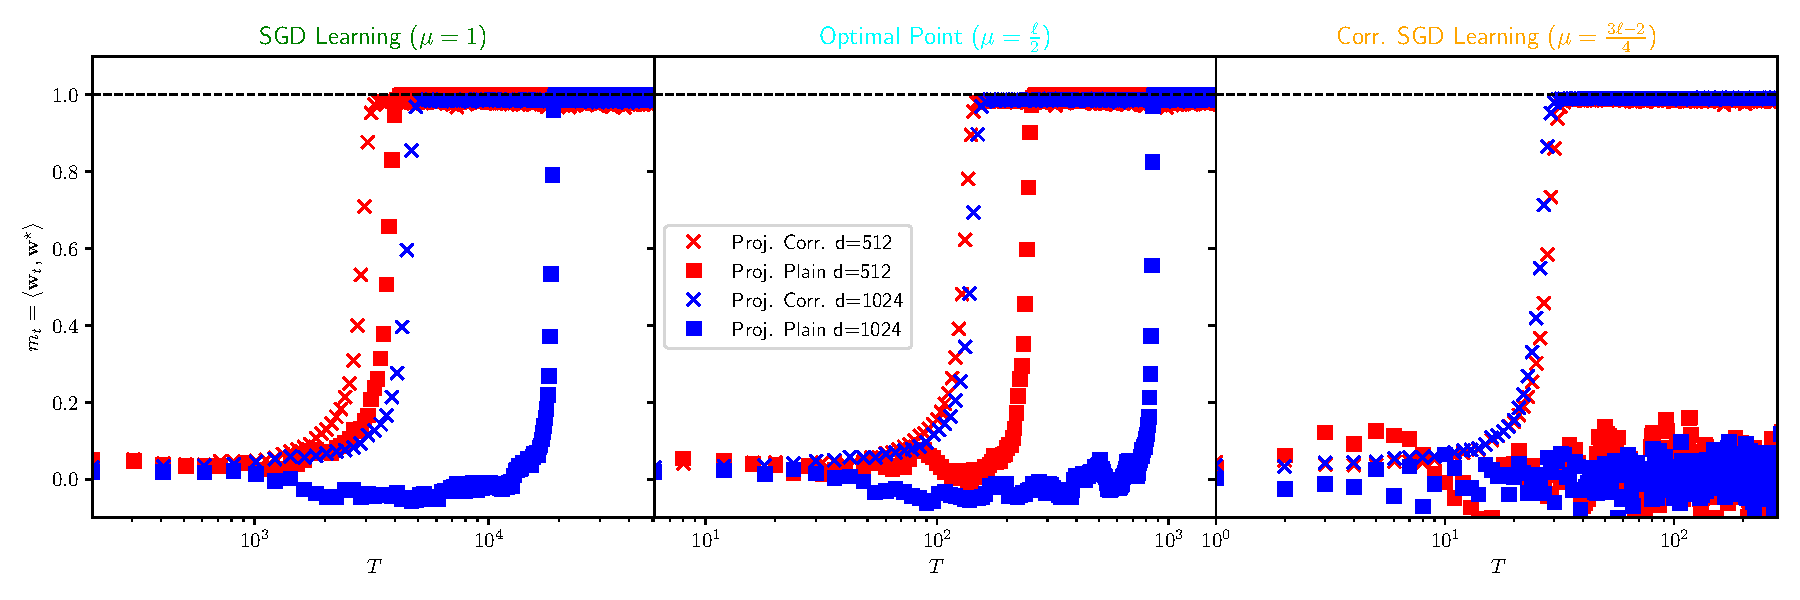
\includegraphics[width=\textwidth, height=0.49\textwidth]{figs/H3H3_m_vs_T}
    \caption{\textbf{{Correlation Loss SGD} weak recovery:} Comparison between the performance of plain SGD and the Correlation Loss SGD, in different regions of the phase diagram, and for different sizes \(d\). The plot shows the test error as a function of the optimization steps. Both the teacher and the student activation functions are fixed to \(\sigma = h^\star =\text{He}_3\), so the information exponent is \(\ell=3\). In all the three plots we vary the value of \(\mu\), while \(\delta = \sfrac{\ell}{2} - \mu\).
    Theorem~\ref{2406:thm:main:no_yhat_weak_recovery} predicts that the \emph{Correlation Loss SGD} weakly recovers the target direction while SGD fails when \(\delta<0\), in accordance to what is shown in the plot. Note that the numbers of steps needed for the target recovery drastically decrease when \(\mu\) becomes large in accordance with Theorems~\ref{2406:thm:main:sgd_weak_recovery},\ref{2406:thm:main:no_yhat_weak_recovery}.
    }
\label{2406:fig:no_yhat_recovery}
\end{figure}
